\documentclass{standalone}
\usepackage{circuitikz}
\usepackage{tikz}

\begin{document}

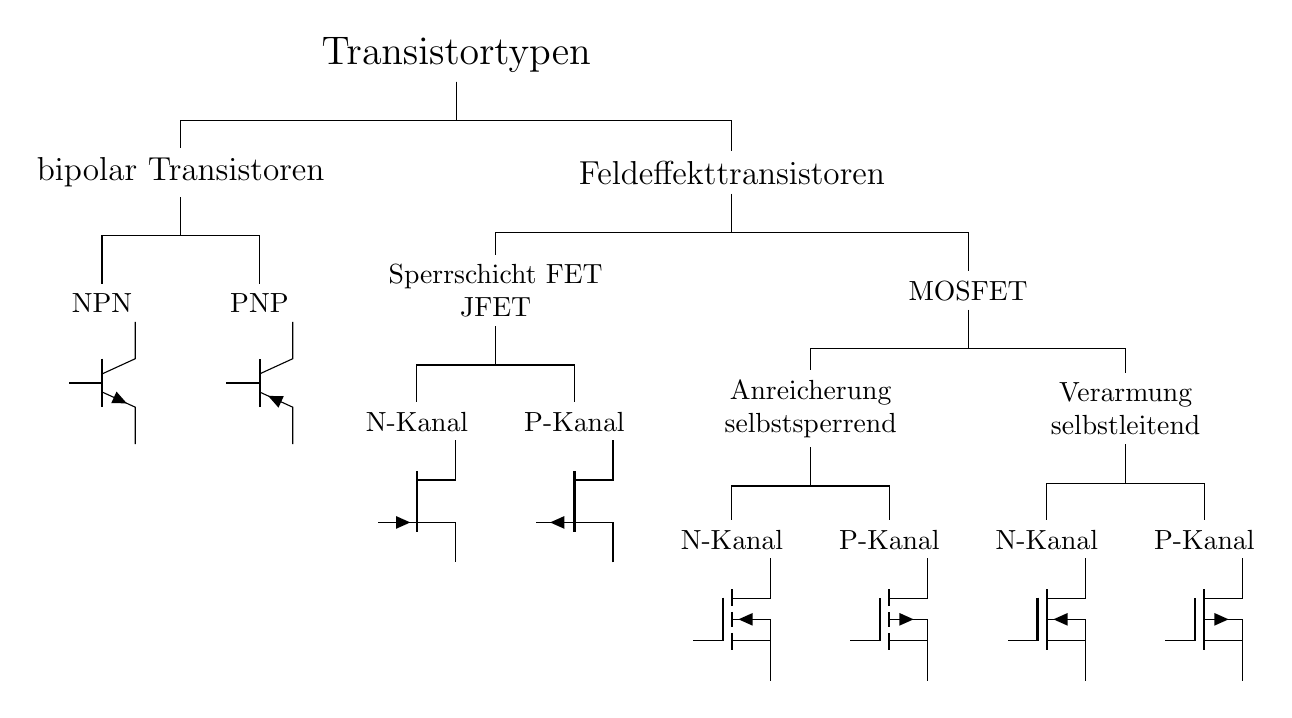
\begin{tikzpicture}

\tikzset{edge from parent/.style={draw,edge from parent path={(\tikzparentnode.south)-- +(0,-14pt)-| (\tikzchildnode)}},
every tree node/.style={align=center,anchor=north}}

\node {\Large Transistortypen}
  [sibling distance=7cm]
  child {node {\large bipolar Transistoren}
  [sibling distance=2cm, level distance=2.5cm]
    child {node {\shortstack{NPN\\\begin{circuitikz}\draw (0,0) node[npn] {};\end{circuitikz}}}}
    child {node {\shortstack{PNP\\\begin{circuitikz}\draw (0,0) node[pnp, yscale=-1] {};\end{circuitikz}}}}
  }
  child {node {\large Feldeffekttransistoren}
    [sibling distance=6cm]
    child {node {\shortstack{Sperrschicht FET\\JFET}}
    [sibling distance=2cm, level distance=2.5cm]
        child {node {\shortstack{N-Kanal\\\begin{circuitikz}\draw (0,0) node[njfet] {};\end{circuitikz}}}}
        child {node {\shortstack{P-Kanal\\\begin{circuitikz}\draw (0,0) node[pjfet, yscale=-1] {};\end{circuitikz}}}}
    }
    child {node {MOSFET}
    [sibling distance=4cm]
        child {node {\shortstack{Anreicherung\\selbstsperrend}}
        [sibling distance=2cm, level distance=2.5cm]
            child {node {\shortstack{N-Kanal\\\begin{circuitikz}\draw (0,0) node[nigfete] {};\end{circuitikz}}}}
            child {node {\shortstack{P-Kanal\\\begin{circuitikz}\draw (0,0) node[pigfete, yscale=-1] {};\end{circuitikz}}}}
        }
        child {node {\shortstack{Verarmung\\selbstleitend}}
        [sibling distance=2cm, level distance=2.5cm]
            child {node {\shortstack{N-Kanal\\\begin{circuitikz}\draw (0,0) node[nigfetd] {};\end{circuitikz}}}}
            child {node {\shortstack{P-Kanal\\\begin{circuitikz}\draw (0,0) node[pigfetd, yscale=-1] {};\end{circuitikz}}}}
        }
    }
  };
\end{tikzpicture}

\end{document}